    %\begin{algorithm}[!t]
%        \centering
%        \caption{Unifying the character font style}
%        \label{alg:unify_font_style}
%        \begin{algorithmic}[1]
%            \REQUIRE~~\\
%                $CI$: Captcha Image  \\
%                $numChar$: The number of characters on Captchas\\
%            \ENSURE~~\\
%                $UC$: Captcha with the same font style \\
%            \STATE $grayCI \leftarrow getBinaryImage(CI)$ \\
%            \STATE $positions[] \leftarrow getHollowPositions(grayCI)$ \\
%            \STATE $LEN \leftarrow getPositonsLen(positions[], numChar)$ \\
%            \STATE $meanThick \leftarrow getMeanCharThick(CI, positions[])$ \\
%            \FOR{$i=1:LEN$}
%                \STATE $cFI \leftarrow FillRedColor(CI, positions[i])$ \\
%                \STATE $cCI \leftarrow ChangeFillColor(cFI, positions[i])$ \\
%                \STATE $charThick \leftarrow getCharThick(cCI, positions[i])$ \\
%                \IF{$charThick>meanThick$}
%                    \STATE $UC=cropChar(cCI, positions[i], meanThick)$ \\
%                \ENDIF
%            \ENDFOR
%        \end{algorithmic}
%    \end{algorithm}
\begin{figure}
  \centering
  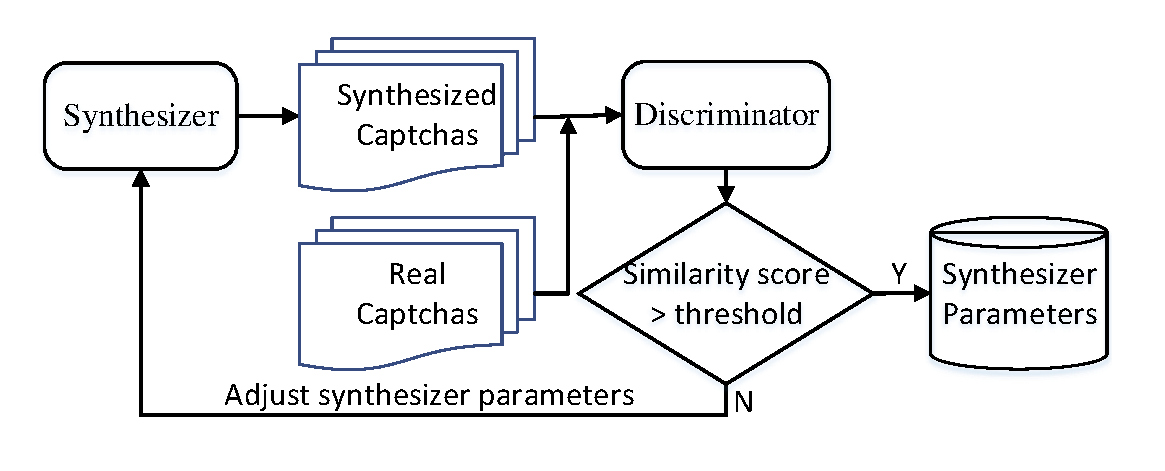
\includegraphics[width=0.45\textwidth]{fig/generator/generator.pdf}
  \caption{This figure shows the overview of captcha generator.}
  \label{fig: generator}
\end{figure}

\section{Implementation Details}
%\section{Captcha Generator} \label{section: Captcha_generator}
A key success factor for deep learning system is large amount of data to train.
Intuitively, the simple yet direct approach in data collecting is to mine the Captchas from target websites and then paid to mark the labels to them artificially. Obviously, it is a time- or financial-consuming work with a high error rate during marking labels. Further, some type of Captchas are difficult to mine as the corresponding websites limit the accessing frequency.
In addition, there is never such a public Captcha generator which can produce enough different styles of Captchas that match the requirement of the training process.
Thus, the first concern of our work is to develop a flexible, well-calibrated training data generator.

To achieve it, we design an generation model to imitate Captchas production process, and automatically generate different styles of Captchas that are similar to those deployed in real-world websites.
Given a unique text-based Captcha scheme $x$, we first manually analyze the number of the characters and their corresponding security features, $S_{1:N}$, with $N$ parameters such as font style, size and color, rotating, distortion and waving \emph{et al.} described in Section~\ref{section: sccturity_features}.
Here we ranked the from No.1 to 10 shown as Table~\ref{table: feature_number}.
We specifics this analysis results as $\{ M, S_{1:N} \}$, where $M$ and $N$ respectively are the number of characters and its styles.
Then given the content of Captcha, our generation model is able to automatically produce Captchas image $y$, which accords with the above analyzed style.
We define our generation model as follows:
\begin{equation}\label{equation: generator_model}
  y \mid x \sim G_s(x),    x = \{M, N, L_{1:M}, S_{1:N} \}
\end{equation}

Where $G_s(x)$ is the generation model parameterized by unique style $s$, that can generate the Captcha image $y$ based on the unique Captcha scheme $x$. $M$ is the number of characters on the Captcha image and $L_{1:M}$ represents the content of the characters. For each character, our generation model individually generates corresponding style defined by $S_{1:N}$, because each character on some Captchas may have different style.

\textbf{Example:} We use the Captcha image depicted in Figure~\ref{fig:overview} as an example to describe our Captcha generator. This Captcha scheme consists of both English letters and Arabic numerals and the number of characters are fixed (4 characters). The content of the Captcha is $\{7, j, R, U\}$.
It uses 2 anti-segmentation features (Complex Background and Connection Lines) and 4 anti-recognition features (Character Set, Font size, Rotating and Distortion). So the collection of security features number is \{\circled{\small 0}, \circled{\small 1}, \circled{\small 3}, \circled{\small 4}, \circled{\small 6}, \circled{\small 7}\}.
Considering these parameters, the variance $x$ is $\{4, 6, \{7, j, R, U\}, \{\circled{\small 0}, \circled{\small 1}, \circled{\small 3}, \circled{\small 4}, \circled{\small 6}, \circled{\small 7}\}\}$.
For each character in the collection $\{4, 6, \{7, j, R, U\}$, our generator product the subgraph correspond to its security features. At last, the generator aggregates the subgraph to produce a Captcha image.


\subsection{Synthesizing Target Captchas \label{section: captcha_generator}}
A key success factor for deep learning system is large amount of data for training. Intuitively, the simple yet direct approach in data collecting is to crawl the real captchas from target websites and then paid to mark the labels to them artificially. Obviously, it is a time- or financial-consuming work with a high error rate especially for manually marking labels. Furthermore, some websites limit the accessing frequency, making it hard to mine their captchas. In addition, there is never such a public captcha generator which can produce enough different styles of captchas that match the requirement of the training process. Thus, the first concern of our work is to develop a flexible, well-calibrated training data generator.

\noindent \textbf{Captcha Generation Approach:}
To generate adequate training samples, we design a generator that can imitate captcha production process, and automatically generate different styles of captchas that are similar to those deployed in real-world websites. Figure~\ref{fig: generator} presents the overview of the generator. The generator is comprised of a synthesizer and a discriminator. The synthesizer is a captcha generation program that can automatically generate the target captchas based on the synthesizer parameters. The discriminator is able to distinguish the generative captcha from the real one according to their similarity. This aims to reduce human involvement during captcha generation so that selecting optimal synthesizer parameters. The synthesizer parameters are the arguments inputting into the synthesizer program. It is a set of values that are abstracted from the security features of captcha.

\noindent \textbf{Quantifying Synthesizer Parameters:}
The original program for generating captchas is stored on the server so that the adversary cannot get it. However, the captcha generation process is that all captchas are generated based on their security features (Section~\ref{section: security_features}), and each security feature can be regarded as an operation that enhancing the security of captcha. Thus, the adversary can imitate this captcha production process to generate target captchas. Before this production process, it is necessary to quantify the security features of the target captcha as the synthesizer parameters. To do so, we set an operation for each security feature of target captcha, and each operation is controlled by a parameter. For example, the rotating angle of Baidu captcha shown in Figure~\ref{fig:text-based captchas} (e) is random but no more than 30 degrees, and so we set this parameter as 30. Note that the parameter will be set null if the target captcha has no the corresponding security feature.

\noindent \textbf{Synthesizer:}
The synthesizer is a program coded by a python script. It mainly consists of some core functions that can perform the operations corresponding to the security features. Given a unique captcha scheme, we first should manually identify how many security features it used. This process is simple yet fast because we just need to set true when a security feature exists and set false when a security feature does not exist. After that, the synthesizer can automatically initialize the parameter value for each security feature. Figure~\ref{fig: captcha_analysis} presents the security features of Baidu captcha and their corresponding initialized parameter values. The purpose of the synthesizer is to select the optimal parameter values so that producing the captchas as likely as the target one. To do so, the synthesizer can iteratively produce a batch size of captchas until the discriminator cannot distinguish the synthesized examples from the real ones. Here we set the batch size to 512 which is found to give good performance in our initial design experiments using Baidu and Microsoft captchas. Furthermore, the grid search method~\cite{Audet2006Mesh} is used to select the optimal parameters.


\noindent \textbf{Discriminator:}
The discriminator is applied to distinguish the synthesized captchas from the real ones. During training, the discriminator inputs a batch of synthesized captchas or real captchas, and it outputs the similarity score comparing to the real captchas. The training process will be terminated when the similarity score is higher than the threshold which is set to 0.95. In our initial experiment, we observed that the local patches we sample from the synthesized captcha have the similar statistics to a real captcha patches. Therefore, differ from the traditional \GANs that exploiting a global discriminator network, we use the discriminator network defined by Shrivastava~\emph{et al.}~\cite{Shrivastava2016Learning} because it performs well when distinguishing the synthesized samples from the real samples.


%Given a unique text-based captcha scheme $x$, we first manually analyze the number of the characters and their corresponding security features, $S_{1:N}$, with $N$ parameters such as font style, size and color, rotating, distortion and waving \emph{et al.} described in Section~\ref{section: sccturity_features}.
%Here we ranked the security features from No.1 to 10 shown as Table~\ref{table: feature_number}.
%We specifics this analysis results as $\{ M, S_{1:N} \}$, where $M$ and $N$ respectively are the number of characters and its styles.
%Then given the content of captcha, our generation model is able to automatically produce captchas image $y$, which accords with its style.
%We define our generation model as follows:
%\begin{equation}\label{equation: generator_model}
%  y \mid x \sim G_s(x),    x = \{M, N, L_{1:M}, S_{1:N} \}
%\end{equation}
%
%Where $G_s(x)$ is the generation model parameterized by the unique style $s$, that can generate the target captcha image $y$ based on the target captcha scheme $x$. $M$ is the number of characters of $x$ and $L_{1:M}$ represents the content of the characters. For each character, our generation model individually generates corresponding style defined by $S_{1:N}$, because each character on some captchas may have different style.

\begin{figure}
  \centering
  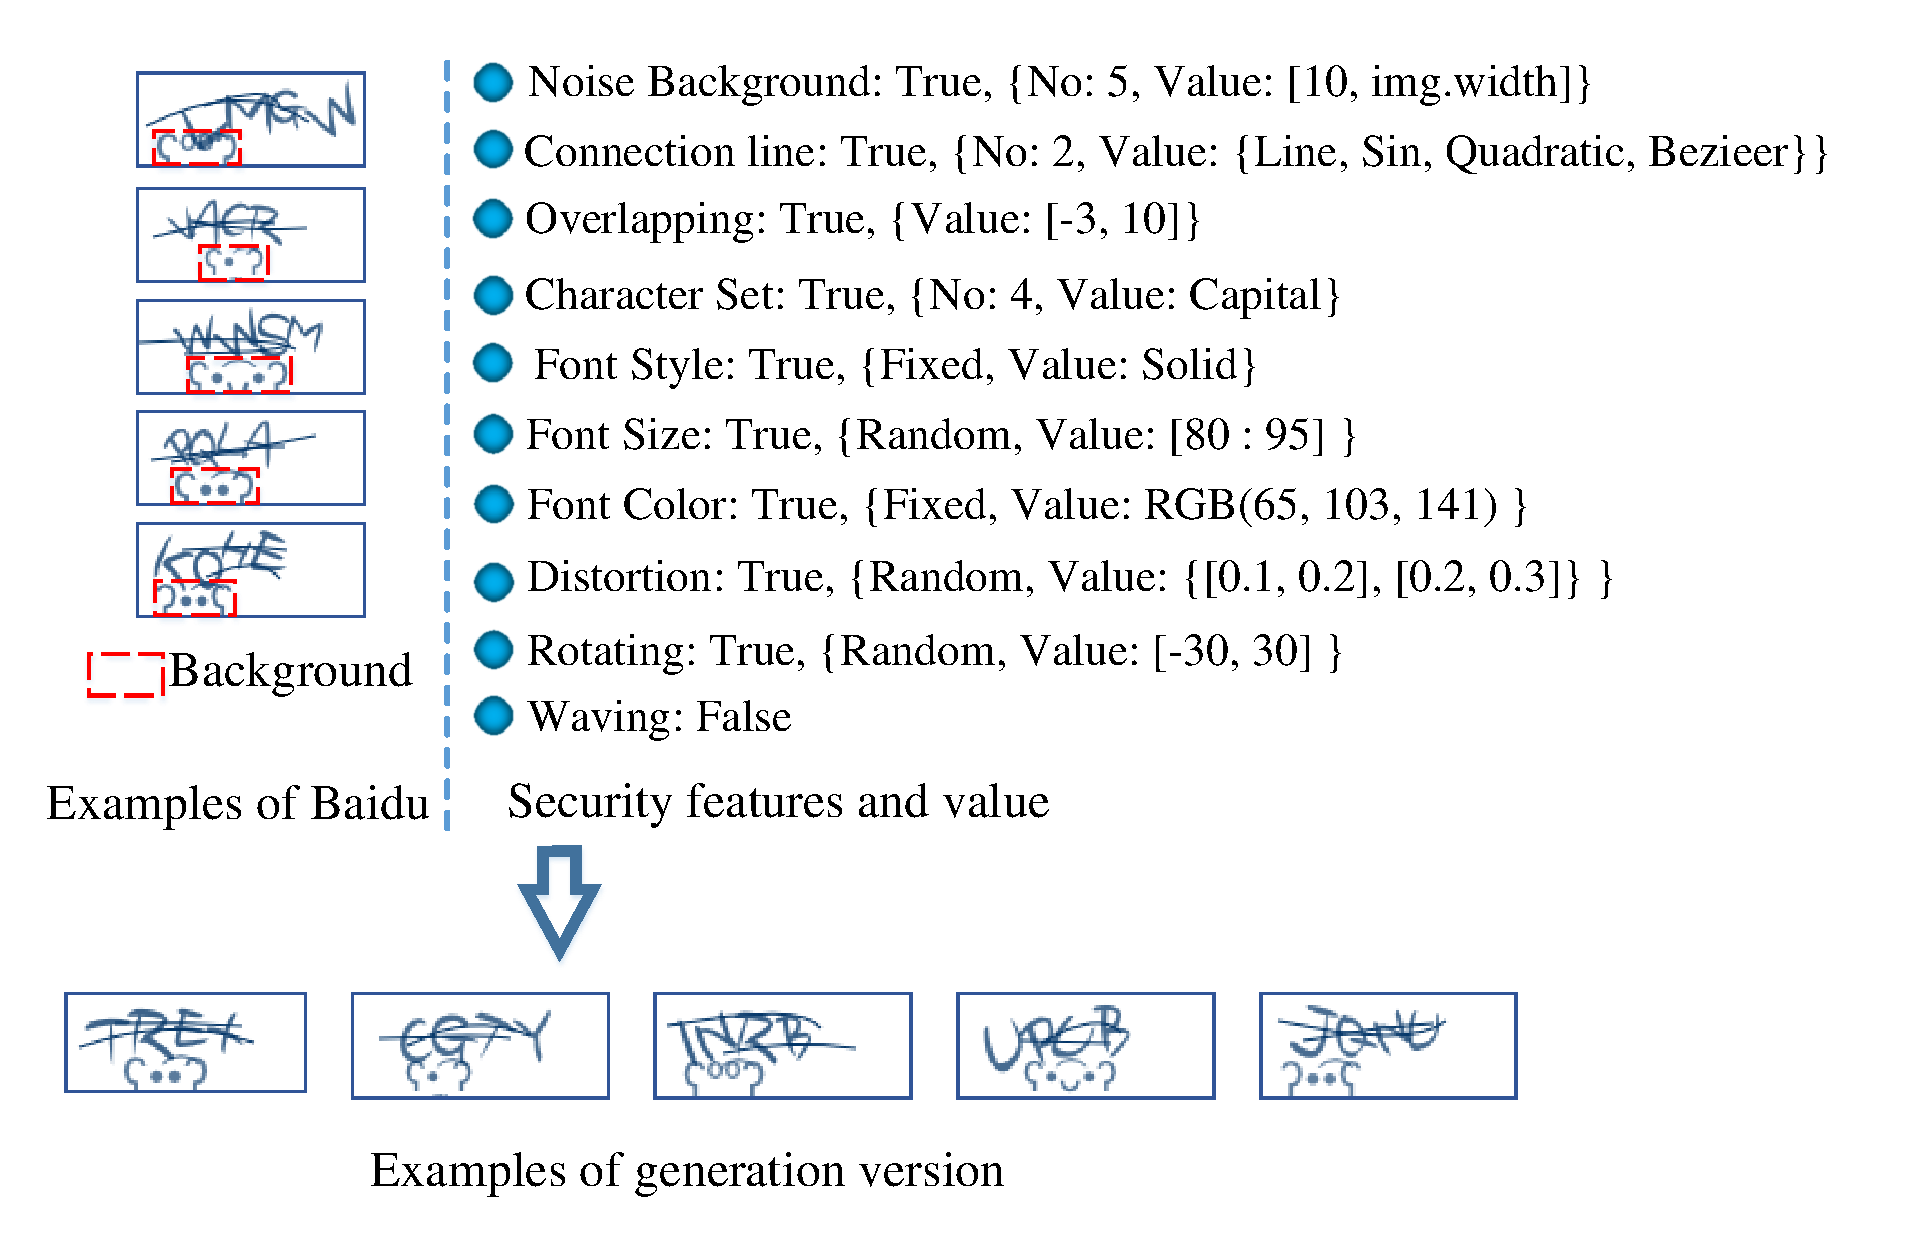
\includegraphics[width=0.47\textwidth]{fig/generator/captcha_analysis.pdf}
  \caption{The figure shows the security features of Baidu captcha and their parameter values.}
  \label{fig: captcha_analysis}
\end{figure}

%\noindent \textbf{Quantify Security Features:} To generate the target captchas as likely as possible, the security features of captcha should be quantified. Given an unique captcha scheme, we first should identify how many security features it used. Then for each used security feature, we need to quantify its parameters value. The last row in Table~\ref{table: feature_number} shows the parameter value for each security feature. For example, if an individual captcha scheme uses rotating and overlapping characters with background, we need to analyze whether the background is fixed or random, the rotating angle and the overlapping distance are fixed or random by observing a number of real captchas. Figure~\ref{fig: captcha_analysis} presents the security features of Baidu captchas and the parameter value of each feature.



\noindent \textbf{Example:}
We use Baidu captcha as an example to describe our captcha generator. This captcha scheme consists of only capital characters with two curves through all four fixed characters and with five kinds of background tricks. Figure~\ref{fig: captcha_analysis} gives the security features of Baidu captcha scheme and their initialized parameter values. From it we can see that Baidu captcha scheme combinates all anti-segmentation features and all anti-recognition features except waving depicted in Section~\ref{section: security_features}. According to the initialization values, the synthesizer first synthesizes a batch of synthesized captchas which are distinguished by the discriminator. If the discriminator can successfully distinguish the synthesized captchas from the real ones, the grid search method is used to select the potential parameter values for synthesizing another batch of captchas. This process will continue iteratively until the discriminator cannot distinguish the synthesized captchas from the real ones. When the process is terminated, the synthesizer will output the optimal parameter values that used to produce the Baidu-like captchas shown in Figure~\ref{fig: captcha_analysis}.
%We use the captcha image depicted in Figure~\ref{fig:overview} as an example to describe our captcha generator. This captcha scheme consists of only English letters and Arabic numerals and the number of characters are fixed (4 characters). The content of the captcha is $\{d, 0, a, A\}$.
%It uses 3 anti-segmentation features (Complex Background, Connection Lines, overlapping) and 4 anti-recognition features (Character Set, Font size, Rotating and Distortion). So the collection of security features number is \{\circled{\small 0}, \circled{\small 1}, \circled{\small 2}, \circled{\small 3}, \circled{\small 4}, \circled{\small 6}, \circled{\small 7}\}.
%Among these security features, we observed that both the location of connection lines and the space of adjacent character are random, and other parameters value of security features are fixed. So the collection of security features can be represented as \emph{SF}: \{\{\circled{\small 0}, f\}, \{\circled{\small 1}, f, r\}, \{\circled{\small 2}, r\}, \{\circled{\small 3}, f\}, \{\circled{\small 4}, f\}, \{\circled{\small 6}, f\}, \{\circled{\small 7}, r\}\}.
%Considering these parameters, the variance $x$ is $\{4, 6, \{7, j, R, U\}, \emph{SF}\}$.
%For each character in the collection $\{4, 6, \{7, j, R, U\}\}$, our generator product the subgraph correspond to its security features. At last, the generator aggregates the subgraph to produce a captcha image.

\begin{figure}
  \centering
  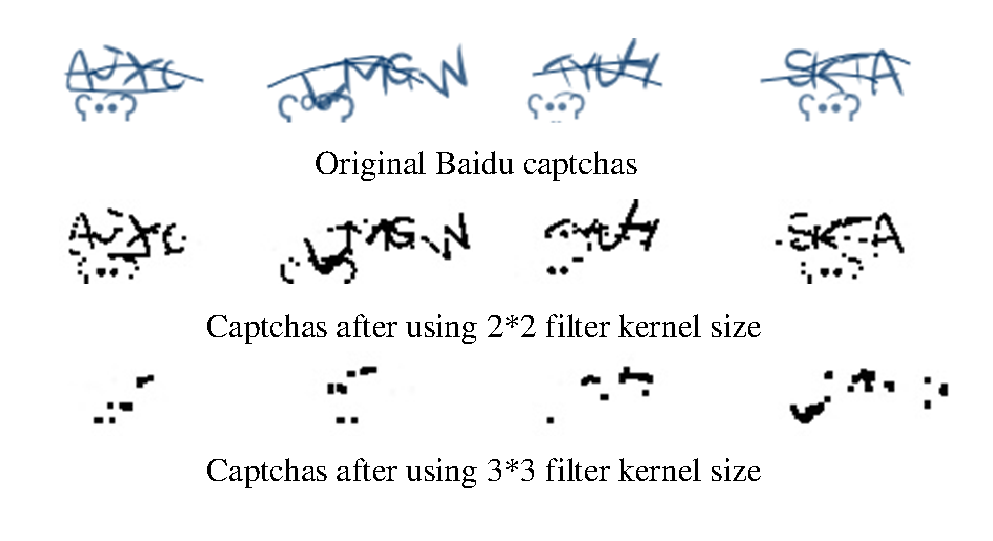
\includegraphics[width=0.47\textwidth]{fig/preprocessing/proofing_removing_background.pdf}
  \caption{The figure shows the results when using different filter kernel size.}
  \label{fig: proofing_removing_background}
\end{figure}

\begin{figure}
  \centering
  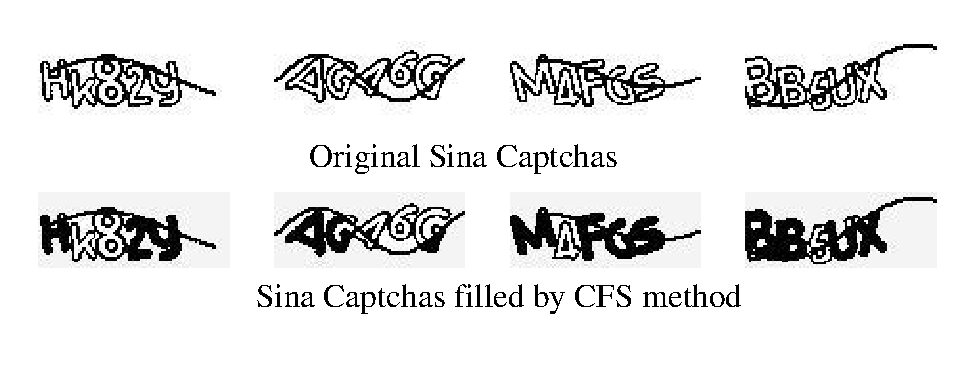
\includegraphics[width=0.5\textwidth]{fig/preprocessing/proofing_cfs.pdf}
  \caption{This figure shows the results of filling the hollow captchas using CFS methods~\cite{Yan2008A}.}
  \label{fig: proofing_cfs}
\end{figure}
%\begin{figure}
%  \centering
%  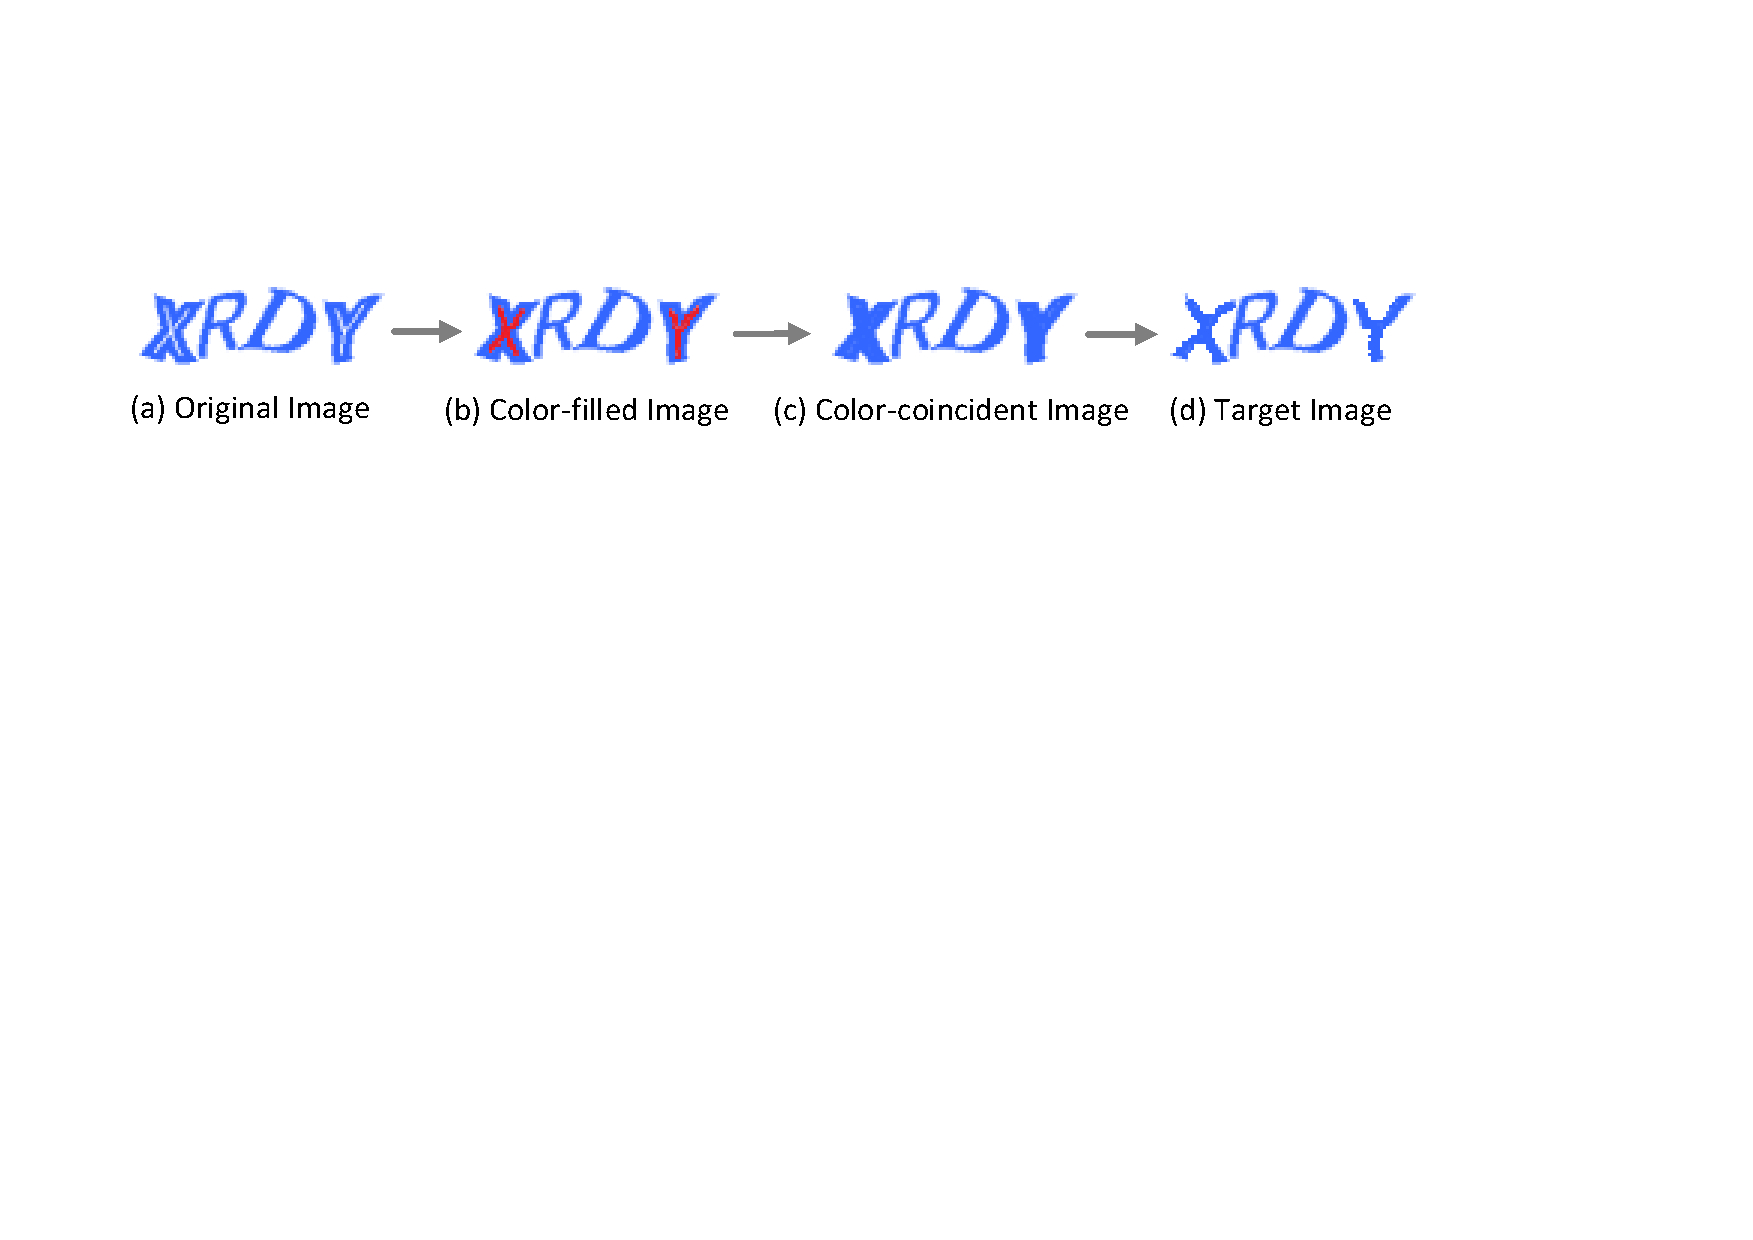
\includegraphics[width=0.5\textwidth]{fig/fill_color.pdf}
%  \caption{The procedure of Captcha preprocessing.}
%  \label{fig:fill_color}
%\end{figure}
%
%\begin{figure}
%  \centering
%  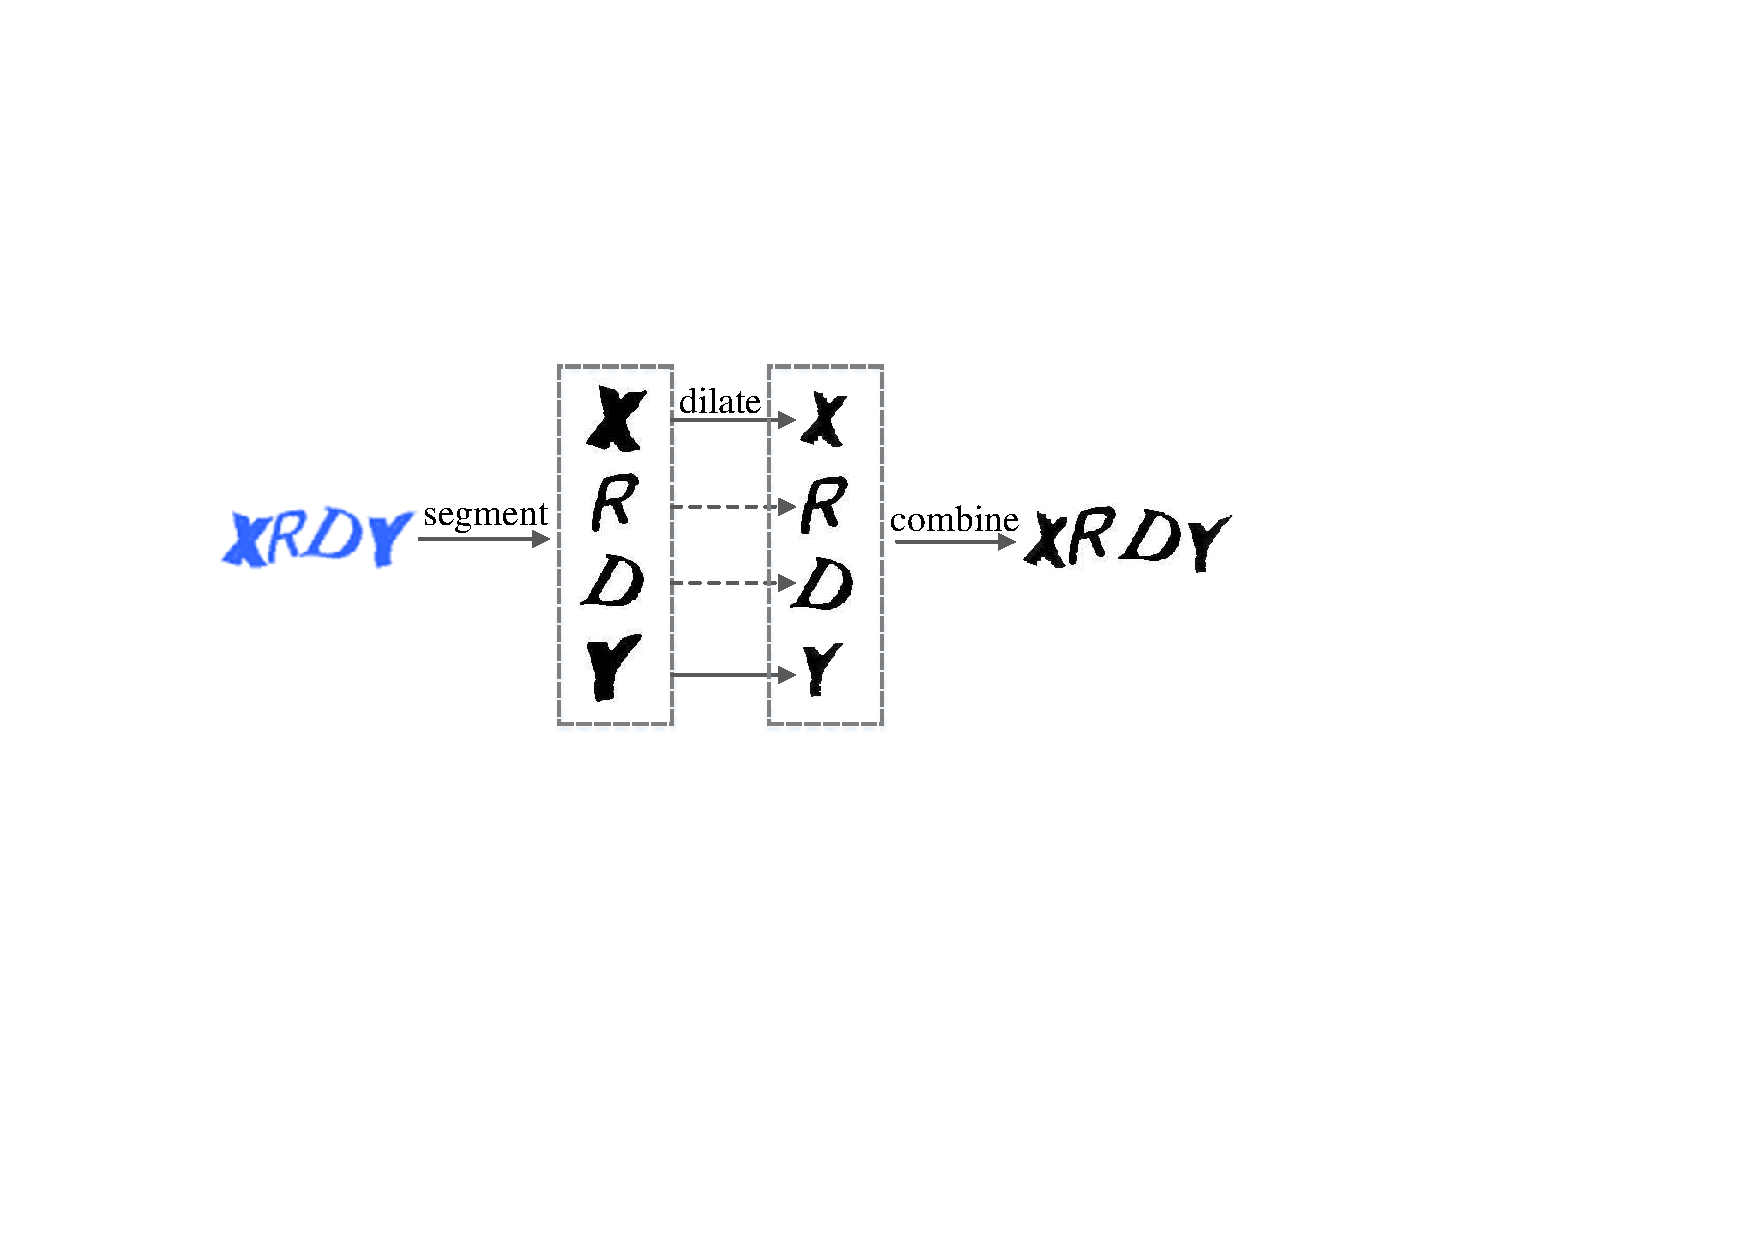
\includegraphics[width=0.45\textwidth]{fig/captcha_preprocessing/preprocessing.pdf}
%  \caption{This figure shows how to unify the font style using the algorithm of morphological dilation.}
%  \label{fig: preprocessing}
%\end{figure}

\subsection{Captcha Preprocessing}
To improve the security of text-based captchas, some schemes contains the following features: (1) noise background or connecting line segments (Figure~\ref{fig: captcha_analysis} (e) and (f)) that can resist segmentation attack; (2) both hollow and solid fonts (Figure~\ref{fig: captcha_analysis} (g)) that increasing the password space so that it is able to defense against recognition. The above two challenges can effectively resist previous segmentation attack. This is proved by the two following proofing experiments: (1) the classic method proposed by~\cite{Yan2008A} fails to removing the connection line of Baidu captchas. This is because the width of the line segments is equal to the width of font so that this method filters out most part of fonts on captchas when using different kernel size of filters as shown in Figure~\ref{fig: proofing_removing_background}; (2) the method of Color Filling Segmentation (CFS) proposed by~\cite{Yan2008A} performs poor when filling the hollow characters of Sina captchas due to the influence of the connection line as shown in Figure~\ref{fig: proofing_cfs}. Furthermore, the CFS method is time-consuming\footnote{It on overage costs 2.5 seconds for filling a Sina hollow captchas.} and it requires adjust many thresholds for each captcha scheme.

Considering the above challenges, we proposed a fast preprocessing approach that can remove the noise background or unify the font styles. We achieve this by employing a variant of image-to-image translation algorithm called \emph{Pix2Pix}~\cite{Pix2PixCode}. This algorithm automatically translates the image from the original style to the target style. In our case, the images to be translated are the captchas with noise background such as Baidu captcha or the captchas with different font styles such as Microsoft captcha. The algorithm aims to remove the noise background or unify the font style of the target captchas. Note that if there is a case that a captcha scheme contains both noise background (or connection line) and different font style such as Sohu captcha (Figure~\ref{fig: proofing_cfs}), our approach will handle this case at the same time.

\noindent \textbf{Variant method of Pix2Pix:}
Like \emph{Pix2Pix}, the method consists of an image generator and a discriminator. They compete with each other until reaching Nash equilibrium during training process. The goal of our method is to construct a generation model that can remove the noise background or unify the font style. In the following, we will introduce our method in detail according to the case of background removal. To build this generation model, we should input the large amount of image pairs. One image pair comprises of one target captcha with noise background and one without noise background. These image pairs are supplied to our method by the synthesizer proposed in Section~\ref{section: captcha_generator}. During building the generation model, the image generator tries to produces the fake captcha that similar to the captcha without noise background by randomly adding the noise points to the original target captcha. The discriminator then will distinguish the fake captchas from the real target ones. The training process will be terminated when the discriminator cannot distinguish the fake captchas. Unlike the \emph{Pix2Pix}, we use the L2 loss function to figure out the loss of the generator because L2 loss function can capturing the overall structure of the captcha image, which contribute to removing the background or unify the font style.

\noindent \textbf{Analysis of Loss Function.}
To demonstrate the effectiveness of L2 over L1 loss function, we conduct many perliminary experiments. Take Baidu captchas for instance, it is expected to be translated to the captchas without noise background or connection lines. When using L1 loss function, some captchas still carries a small number of noise background or connection lines shown as Figure~\ref{fig: L1_L2} (b). In contrary, the noise background and connection lines are cleaned out (Figure~\ref{fig: L1_L2} (c)) when using L2 loss function. This is because the generation model can achieve global optimum when using L2 loss function. Figure~\ref{fig: loss_anlysis} shows that the loss value of L1 has been fluctuating while the value of L2 has been tending to convergence.

%Given some current text-based captcha schemes mainly consist of both solid characters and hollow characters (see Figure~\ref{fig:text-based captchas} (j) and (k)), the first step of our attack is to unify the different font styles to a fixed style. Here we aims to fill the hollow character with solid core due to the following two reasons:
%(1) the hollow character can be easily transformed to the solid one but not the opposite.
%(2) the solid character can be extracted more stable features than hollow character at the following step according to our preliminary experiments.
%
%To do so, we first convert the colorful image to black-and-white using the standard threshold selection method proposed by Otsu~\cite{Ostu1979A}\footnote{Note that we only use the binarized image to locate the position of the hollow part of the character other than furthering processing.}.
%Then the Color Filling Segmentation (CFS)~\cite{Yan2008A} is used to fill the hollow character with the red color (see Figure~\ref{fig:fill_color} (b)). Next, the color-filled image should be convert to color-coincident image by changing the red filled area to the original character color (see Figure~\ref{fig:fill_color} (c)). At last, the thick filled characters on the color-coincident image need to be cropped as the original character (see Figure~\ref{fig:fill_color} (d)).
%
%However, how to translate the color-coincident image to the target image (shown in Figure~\ref{fig:fill_color}) is a challenge. Fugure~\ref{fig: preprocessing} presents our approach to address this challenge. We first segment the characters using CFS method~\cite{Yan2008A}.  Then we extract the color-filled characters and using morphological algorithm to dilate these characters. To effectively dilate both the edge and inflexion areas, we use the ellipse and cross kernels. We set the size of the kernel to (10, 10), an empirical setting that makes dilated characters clearly visible. After that, we combine these segmented characters to a captcha image.
%
%Our method for unifying the character font style is described in Algorithm~\ref{alg:unify_font_style}.
%The input to the algorithm is the original captcha image with different font styles and the number of characters on this captcha, and the output of the algorithm is the captcha with solid characters. To locate the hollow characters, we first convert the colorful original image to binarized image (line 1). According to the binarized image, we can get the positions of the each hollow characters on the colorful captcha image (line 2) because the size of colorful image is the same as the binarized image. For each hollow character, we use CFS method described above to fill it with red color (line 6) and then replace the red filled color with the character color to get the color-coincident image (line 7). Finally, we crop the filled character on the color-coincident image to unify the font style of characters (line 10).

\begin{figure}
  \centering
  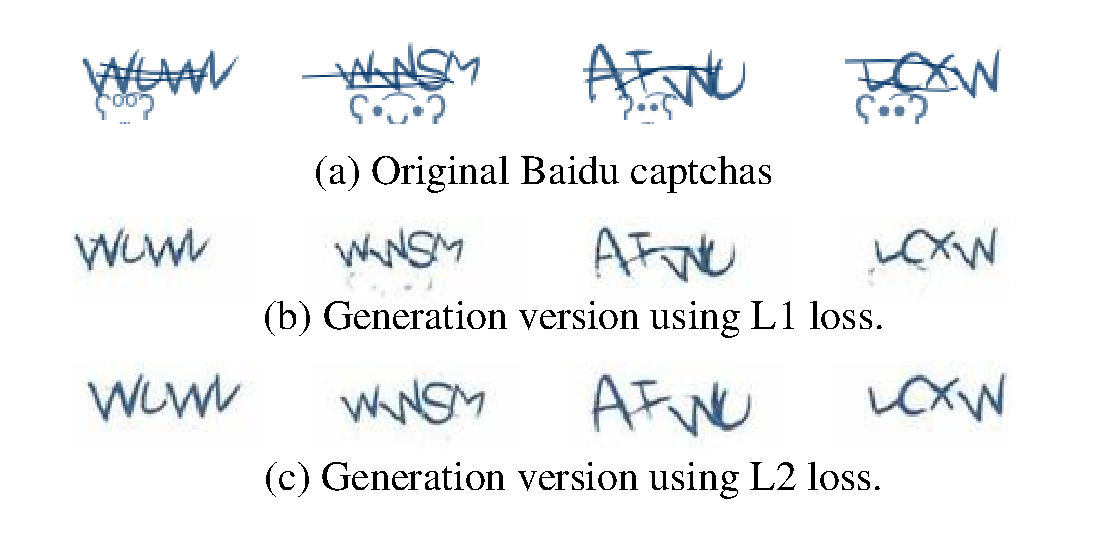
\includegraphics[width=0.45\textwidth]{fig/preprocessing/captcha_generated.pdf} \\
  \caption{Captchas generated when using L1 and L2 loss function.}
  \label{fig: L1_L2}
\end{figure}

\begin{figure}
  \centering
  \subfigure{
      \begin{minipage}[t]{0.22\textwidth}
      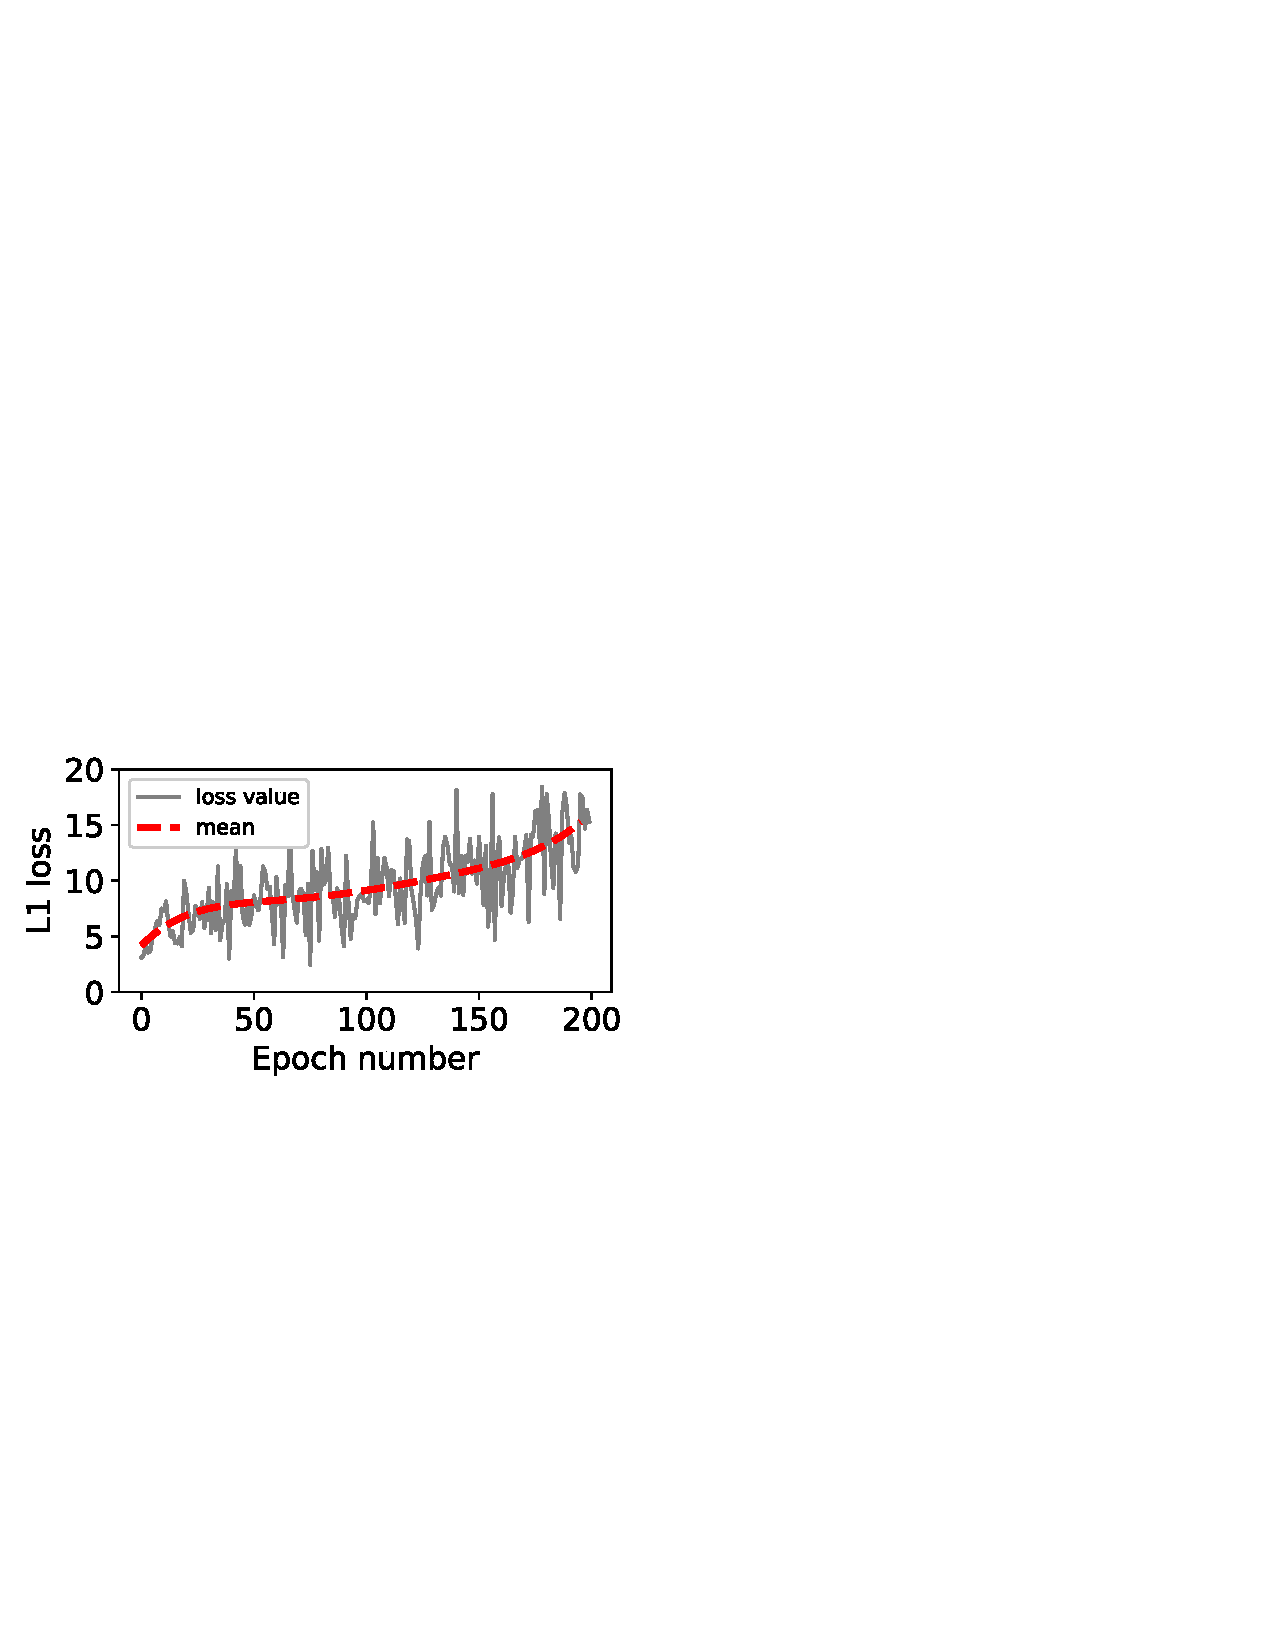
\includegraphics[width=\textwidth]{fig/loss_anlysis/loss_L1.pdf}\\
      \center L1 loss curve
      \end{minipage}
  }
  \subfigure{
      \begin{minipage}[t]{0.22\textwidth}
      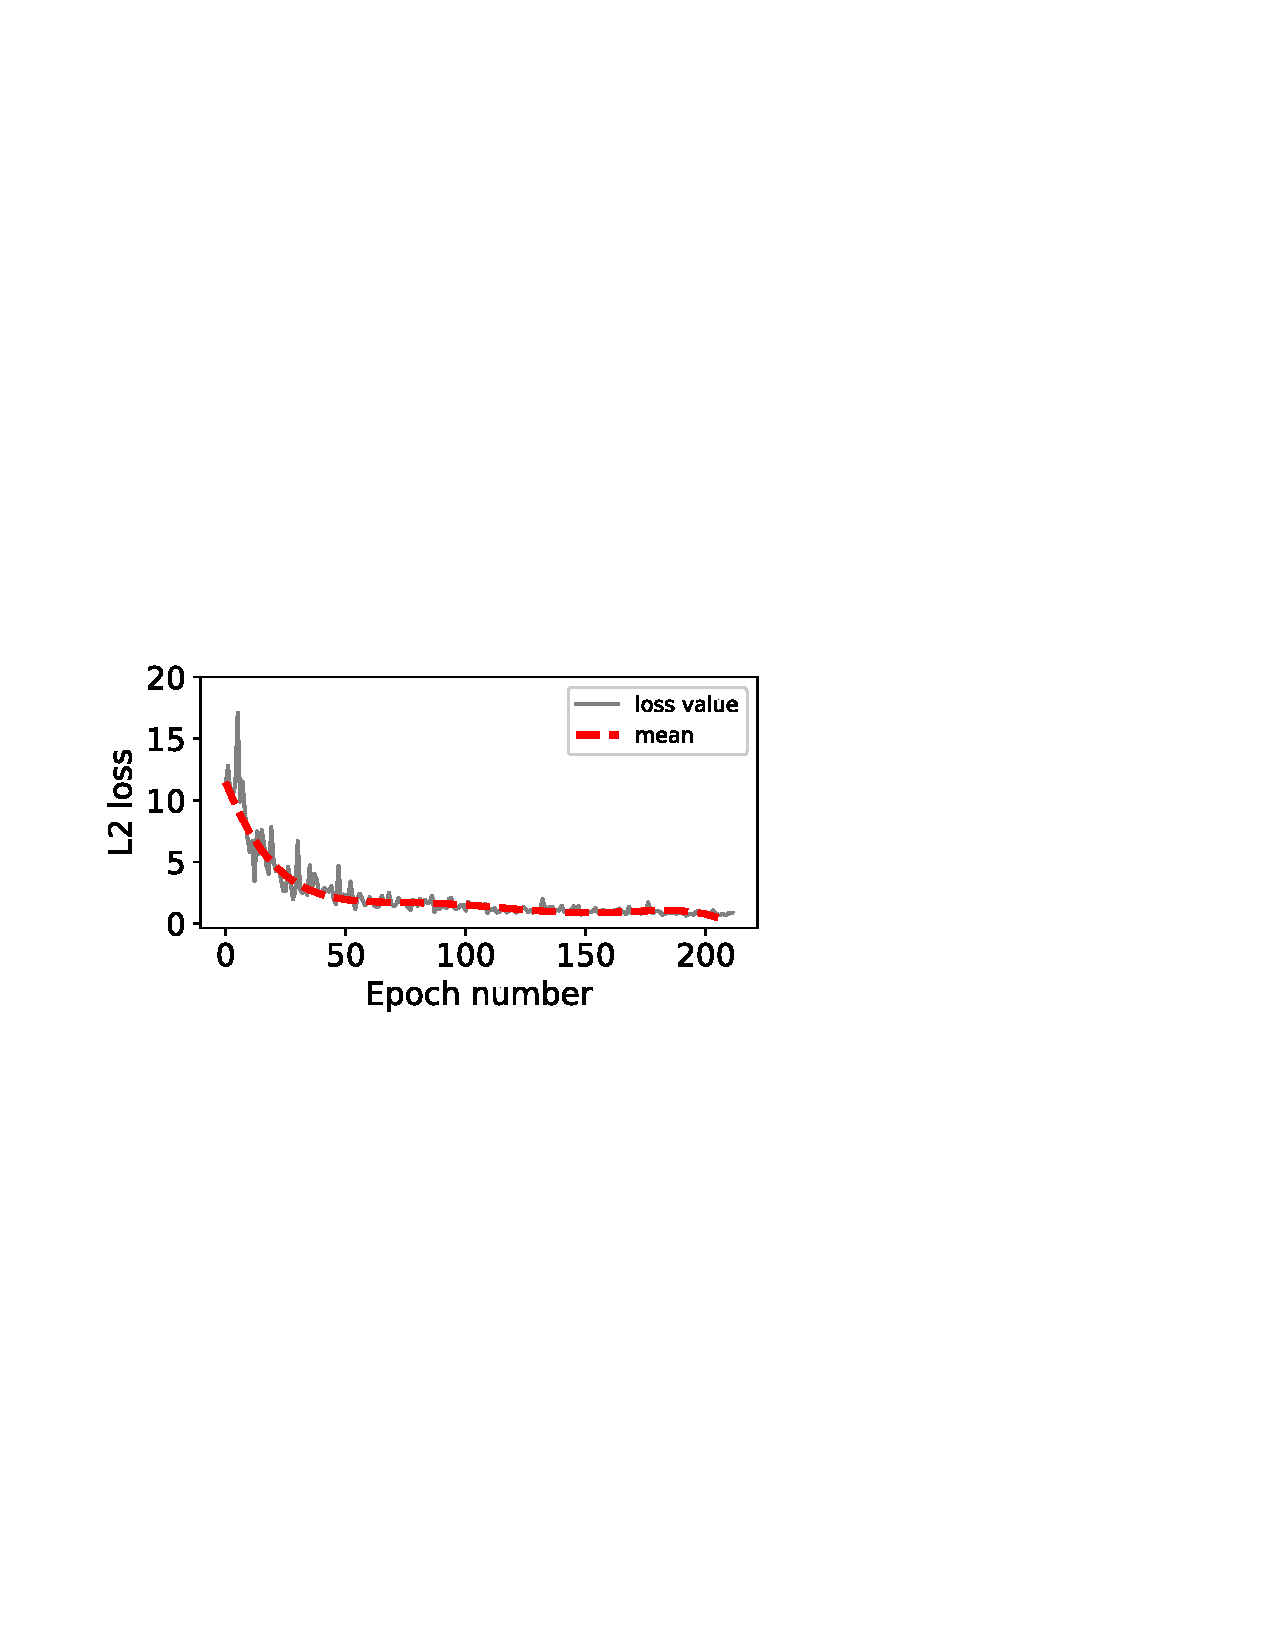
\includegraphics[width=\textwidth]{fig/loss_anlysis/loss_L2.pdf}\\
      \center L2 loss curve
      \end{minipage}
  }
  \caption{This figure shows the L1 and L2 loss curve when train using captcha scheme in Figure~\ref{fig: L1_L2}.}
  \label{fig: loss_anlysis}
\end{figure}

%\subsection{Generate Regular Captcha}
%After unifying the character font style, we need to generate regular captchas for further recognizing. We achieve this by employing an image-to-image translation algorithm called~\emph{Pix2Pix}~\cite{Pix2PixCode}. This algorithm automatically translate the image from the original style to the target style. In our case, the images to be translated are the captchas with complex noisy background, overlapping and distorted characters (original style). These are supplied to the algorithm by a captcha generator developed using a simple script (Section~\ref{section: Captcha_generator}). The algorithm tries to generate regular captcha with appropriate character spacing and clean background (target style).
%Note that if the captcha to be translated has no background as Google scheme (Figure~\ref{fig:text-based captchas} (l)), our approach just enlarge the space of adjacent character and Regularization operations. Likewise, if the captcha only contains deformed but no overlapping characters (Figure~\ref{fig:text-based captchas} (j)), our approach only need to regular the characters.
%
%\noindent \textbf{Hierarchical Methods.} In order to generate regular captcha, we propose a hierarchical method that employ a variant approach of \emph{Pix2Pix} to complete the progressive tasks.
%The hierarchical methods are comprised of three sequenced models, and they can respectively achieve three different tasks: removing complex background, expanding space of adjacent overlapping characters and making the distorted character to be a regular one. These three sequence models share the same methodology of~\emph{Pix2pix}.
%The main differences of these sequences models are the input and output.
%The output of the previous model is the input of the following model.
%Take the captcha in Figure~\ref{fig:overview} for an example, the first model is applied to eliminate the complex background and Connecting lines and output the captcha with clean background. Then the space of the characters on the output captcha is expanded by the second model, and produces the captcha only with distorted characters. Finally, the distorted characters are translated to the regular ones using the last model.
%%The inputs of the first step are the images with complex background, overlapping and distorted characters.
%%These inputting images are eliminated the complex background by the variant approach which outputs the Captcha images with clean background, overlapping and distorted characters.
%%According to the outputs, the second step is to expand the space between the adjacent overlapping characters using the same variant method, and produces the Captcha images only with distorted characters.
%%Finally, the distorted characters are translated to the regular ones using the variant method.
%
%\noindent \textbf{Key Algorithm.} The key part of the hierarchical methods is a variant of \emph{Pix2Pix}. It consists of an image generator and an discriminator. They are competing with each other until reach Nash equilibrium during training processing (Section~\ref{section: GANs}).
%We take the generation model of removing complex background for detailed introducing our key algorithm.
%The goal is to train a generative model that can translate the captcha image with complex background to the images with clean background.
%In order to train this generation model, the input data are the image pairs including the captcha images with background and the images with clean background.
%During training, the image generator produces the fake image that similar to the image with white background by randomly adding the noisy points to it. The fake image and the image with complex background compose an image pair.
%For the composed image pair, the discriminator learns to classify between the real and fake pairs. This competing process will be terminated until the discriminator cannot correctly classify the image pairs.
%Unlike the \emph{Pix2Pix}, we use the L2 loss function to figure out the loss of the generator because L2 loss function can capturing the overall structure of the captcha image, which contribute to removing the background and other two tasks (expand the space of adjacent characters and eliminate distorted characters).
%\begin{equation}\label{equation: L2_loss}
%    \mathcal{L}_{L2}(Gen) = \mathbb{E}_{x,y \epsilon C_{O}, z \epsilon N_{O}} \|y - Gen(x, z)\|_{2}
%\end{equation}
%
%Where $x$ is the captcha image with white background, $y$ is the image with complex background and $z$ is the fake image with the noisy points.
%
%\noindent \textbf{Analysis of Loss Function.} To demonstrate the effectiveness of L2 over L1 loss function, we conduct many perliminary experiments. Take Figure~\ref{fig: L1_L2} (a) for instance, it is expected to be translated to regular Captcha as Figure~\ref{fig: L1_L2} (b). When using L1 loss function, only one character can be successful translated to the target one shown as Figure~\ref{fig: L1_L2} (c). In contrary, all characters can be correctly translated to be the regular ones (Figure~\ref{fig: L1_L2} (d)) when using L2 loss function. This is because the generation model can achieve global optimum when using L2 loss function. Figure~\ref{fig: loss_anlysis} shows that the loss value of L1 has been fluctuating while the value of L2 has been tending to convergence.

%The hierarchical methods are comprised of three sequenced models, and they can respectively achieve the tasks of removing complex background, expanding space between adjacent overlapping characters and translating the distorted Captcha to a regular one. The sequenced models share the same translation model.
%The key part of the translation model is a variant of \emph{Pix2Pix}, which consists of a image generator and discriminator. They are competing with each other until reach Nash equilibrium when training processing (Section~\ref{section: GANs}).
%
%In our case of removing background, the inputting data are the image pairs including the Captcha images with complex background and the images with white background.
%The goal is to train a generative model that can translate the Captcha image with complex background to the images with white background.

\begin{figure}[!t]
  \centering
  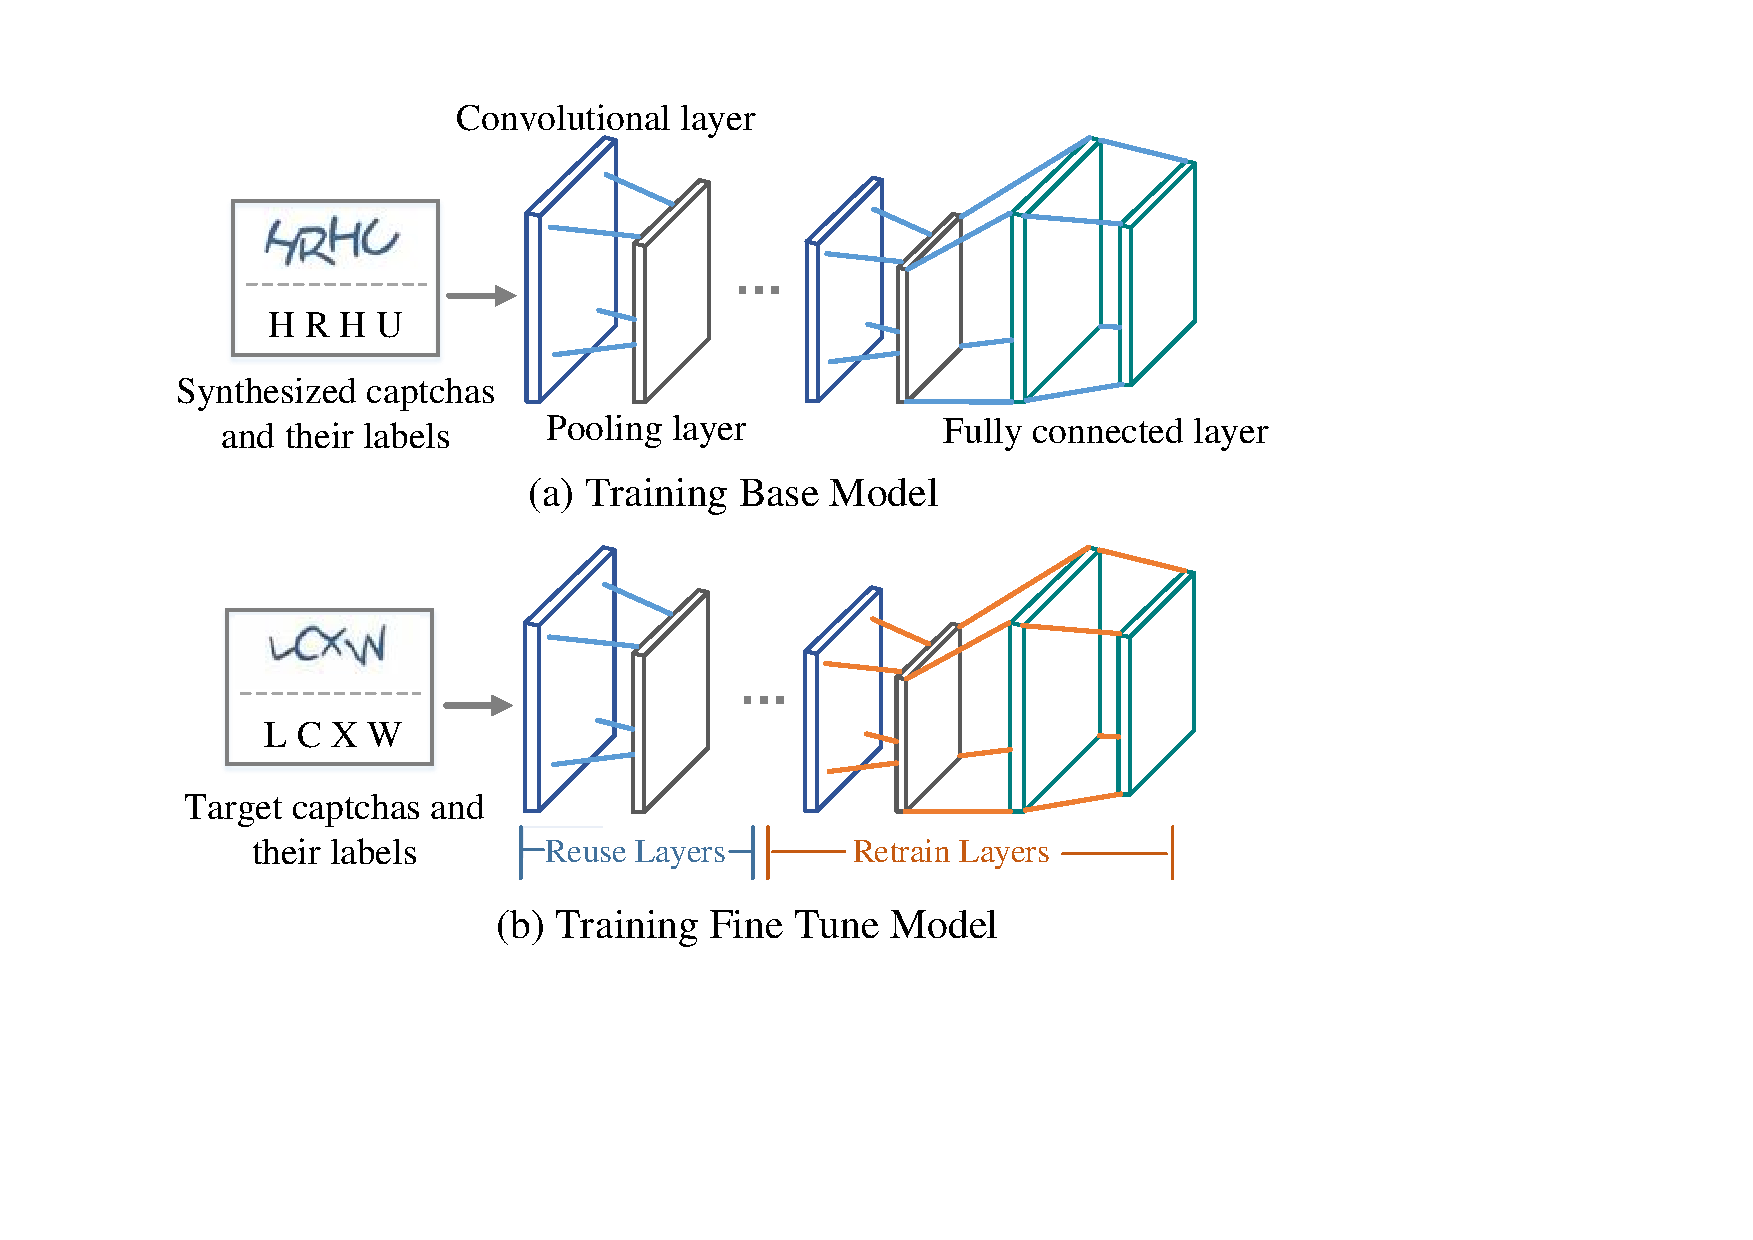
\includegraphics[width=0.45\textwidth]{fig/cnn_model.pdf}
  \caption{The overview of base model and fine tune model. We use large amount of synthesized captchas to train the base model shown in (a). (b) presents that we reuse the former 4 layers of the base model to build the fine tune model through using a number of real target captchas.}
  \label{fig: cnn_model}
\end{figure}

\subsection{Identify Captcha}
In this step, we use a rudimentary CNN framework, \emph{LeNet-5}~\cite{Lecun1998Gradient}, as our recognition engine, to build the based model and fine tune model for identifying the target captchas.
The initial \emph{Lenet-5} was compromised of three convolutional layers, two pooling layers and followed by two fully connected layers.
The convolutional layer extracts the features using a number of filters that are trained during training process. The pooling layer aggregates the features extracted from the convolutional layer for extracting more representative features meanwhile reducing the amount of calculation. The fully connected layer classify the extracted features into target categories. The appropriate number of network layers determines the quality of the extracted features as proper number of layers will extract more representative features.

\noindent \textbf{Base Model:}
Unlike the \emph{LeNet-5}, the goal is to recognize the captchas, which is more difficult than recognition a single character done by \emph{LeNet-5}. This is because recognizing more characters need to extract more complex and abstract features. Therefore, a more complex base model is needed for building effectively fine tune model.
To do so, we redesign the \emph{LeNet-5} and adding another two convolution layers and another three pooling layers.
Figure~\ref{fig: cnn_model} (a) depicts the framework of our base model. Generally, it consists of five convolution layers, five pooling layers and followed by two fully connected layers. Each convolution layer is followed by a pooling layer.

To extract more representative features, each convolutional layer uses a convolution filter of $3 \times 3$ and each pooling layer employs the max-pooling value. Other parameters are the same as the \emph{LeNet-5}.

\noindent \textbf{Fine Tune Model:}
Although our synthesizer can produce the captchas similar to the target ones, the inevitable difference between the synthesized captcha and the real one still exists. To relieving this difference, we use transfer learning method to build the fine tune model based on the base model. During transferring the model, we keep the parameters of the former 4 layers and retrain the parameters of remaining layers. Figure~\ref{fig: cnn_model} (b) presents the fine tune model.










